\documentclass[11pt,a4paper]{article}
\usepackage[utf8]{inputenc}
\usepackage[english]{babel}
\usepackage{amsmath}
\usepackage{amsfonts}
\usepackage{amssymb}
\usepackage{graphicx}
\graphicspath{{../figures/}}
\author{Jacob Heden Malm}
\title{DD2424 Assignment 1}
\begin{document}
\maketitle

\section{Implementation details and success of gradient descent}

I was able to write all of the required functions without issue. In order to verify that my gradient computations were correct, I first debugged the program during its execution and visually compared the gradient values computed by my gradient descent method as well as the numerical approximation method we were given. I then wrote a method called "verify\_gradient\_descent()" that a mini batch of training examples, the weight and bias matrix, a regularization parameter, and a permitted difference. This method then computes the gradient update using the analytic method and the numerical method, and takes the absolute value of the difference matrix computed by the two methods. It then asserts that the means of these two matrices (W and b) are less than the permitted difference parameter. Using a mini batch of 5 data points, and a regularization multiplier of 0.01 I got the mean of the absolute difference to be in the neighborhood of 4.5e-8. I took this to signify success.\\

I also chose to randomize the order of training examples between each epoch.

\section{Data and figures}
Here, graphs detailing the training development and images representing the learnt weight matrix will be shown for the different required parameter settings.

\subsection{$lambda=0$, $eta=0.1$}
Final test accuracy: 0.3027

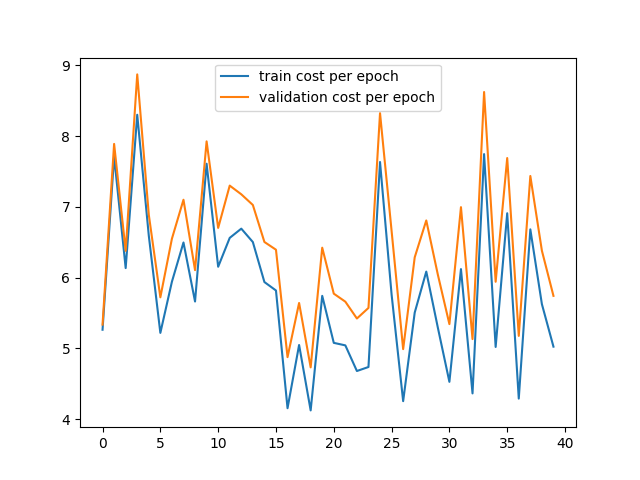
\includegraphics[width=\textwidth]{eta_0.1_lambda_0.png}
As we can see the learning rate here is much too high. This leads to the network never really learning any useful parameters, each new training example changes the parameter settings too much for the network to retain any "knowledge" it has gained from previously seen training examples.

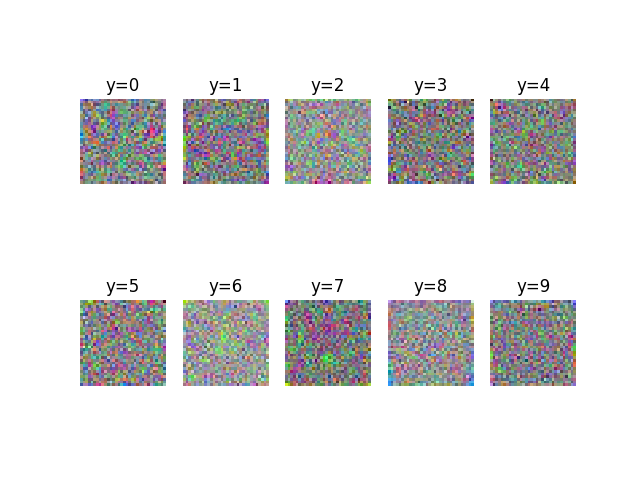
\includegraphics[width=\textwidth]{eta_0.1_lambda_0_montage.png}

These images do not tell us much, they seem to be relatively random blobs of color.


\subsection{$lambda=0$, $eta=0.001$}
Final test accuracy: 0.4097

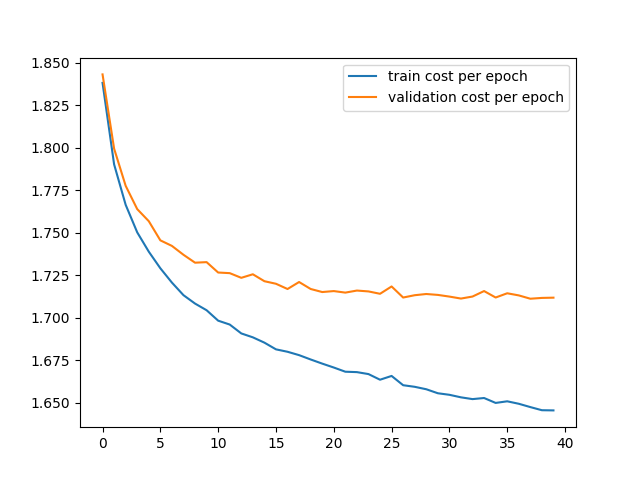
\includegraphics[width=\textwidth]{eta_0.001_lambda_0.png}

Here we can see that this learning rate seems to be a better fit for this network and training data. Especially the training loss seems to decrease steadily as training continues, suggesting that the network continues to get more and more fitted to the training examples we give it.

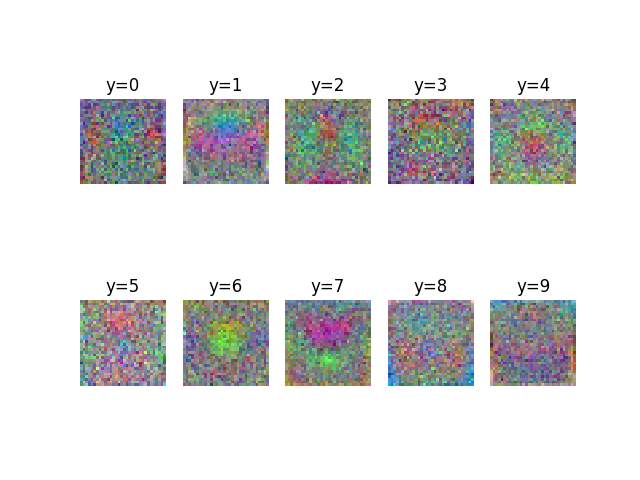
\includegraphics[width=\textwidth]{eta_0.001_lambda_0_montage.png}

We can see clear shapes begin to take form in the learned weight matrix.

\subsection{$lambda=0.1$, $eta=0.001$}
Final test accuracy: 0.4095

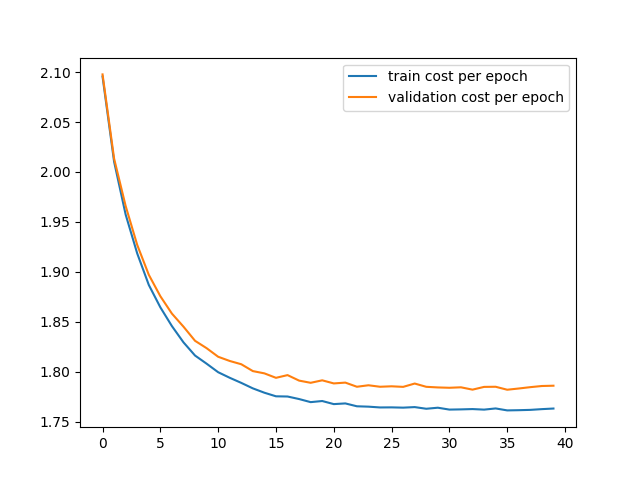
\includegraphics[width=\textwidth]{lambda_0.1.png}

Here we can see the effect of added regularization. Regularization decreases the networks variance, which combats its tendency to overfit. This is demonstrated in the much smaller discrepancy between the networks training and validation loss than in the previous example.

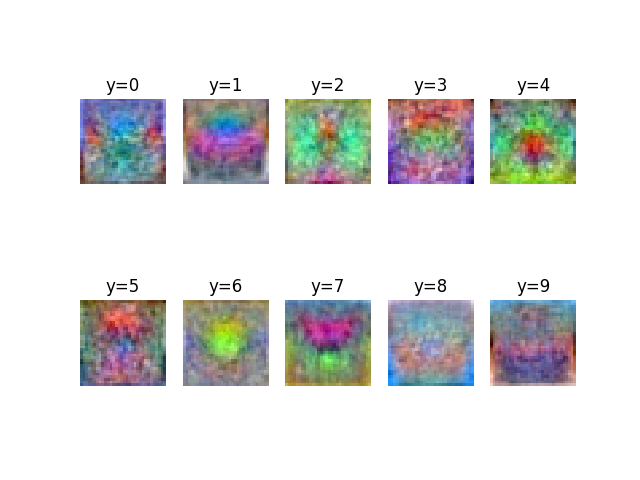
\includegraphics[width=\textwidth]{lambda_0.1_montage.png}

Compared with the previous example, these images look much clearer. The validation accuracies are however more or less equivalent, personally I am not sure how regularization achieves this. Perhaps since increasing the amount of regularization encourages a smoother output function, this results in clearer regions of uniformity in the generated images, essentially encouraging spatial correlation in the pixel values.

\subsection{$lambda=1$, $eta=0.001$}
Final test accuracy: 0.3801

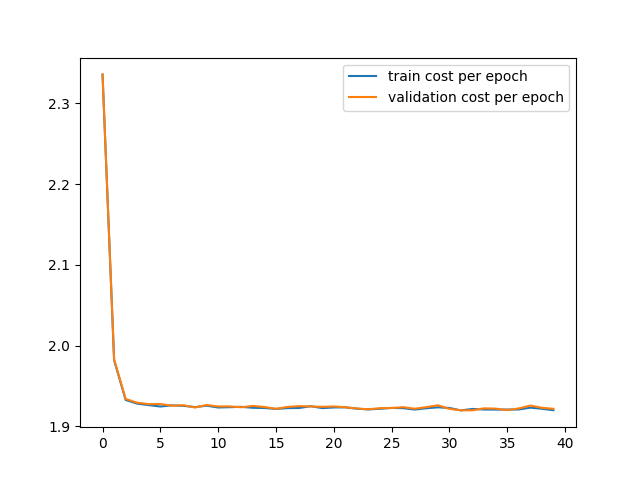
\includegraphics[width=\textwidth]{lambda_1.png}

The aforementioned effects are much more pronounced here. It is however also notable that the loss never reaches as low as it did in the previous example, suggesting that this amount of regularization has introduced too much bias.

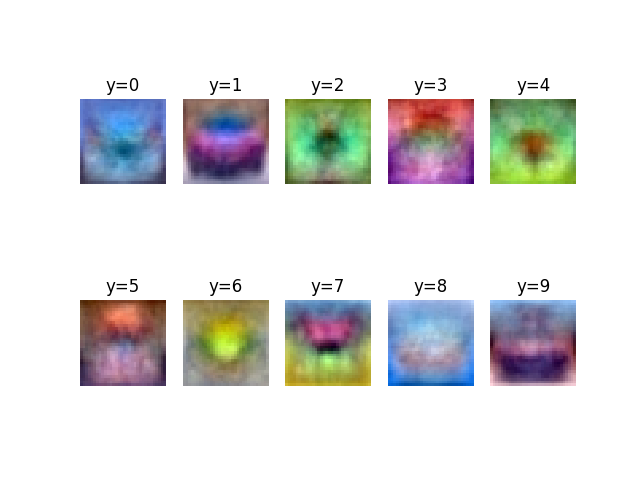
\includegraphics[width=\textwidth]{lambda_1_montage.png}

These images actually look quite good! The lack of noise makes them quite visually appealing in comparison to the previous images. However, noticeably, the test accuracy of this parameter setting is lower than the previous example.

\end{document}